\documentclass{beamer}
\usepackage{csquotes}
\usepackage{tikz}
\usetikzlibrary{arrows,positioning,shapes.geometric, calc}
\usepackage{amsmath}
\usepackage{listings, xcolor}
\usepackage{lmodern}
\usepackage{adjustbox}
\usepackage{booktabs}
\usepackage{colortbl}
\usepackage{caption}
\usepackage{icomma}
\usepackage{bigstrut}
\usepackage{geometry}
\usepackage{subfigure}


\usetheme{metropolis}           % Use metropolis theme
\title{Spark and Hail: An Introduction}
\date{\today}
\author{Robert M. Porsch}
\institute{Center of Genomic Science}
\begin{document}
\maketitle

\begin{frame}
  Main aim of this presentation
  \begin{itemize}
    \item What is Spark and why is it useful?
    \item Hail: Spark for genetic data analysis
    \item The cloud: Experiences using Hail after 2 weeks
  \end{itemize}
  Bonus: Distributed statistical learning
\end{frame}

\begin{frame}{Basic Architecture of Spark}
  \begin{figure}
    \centering
    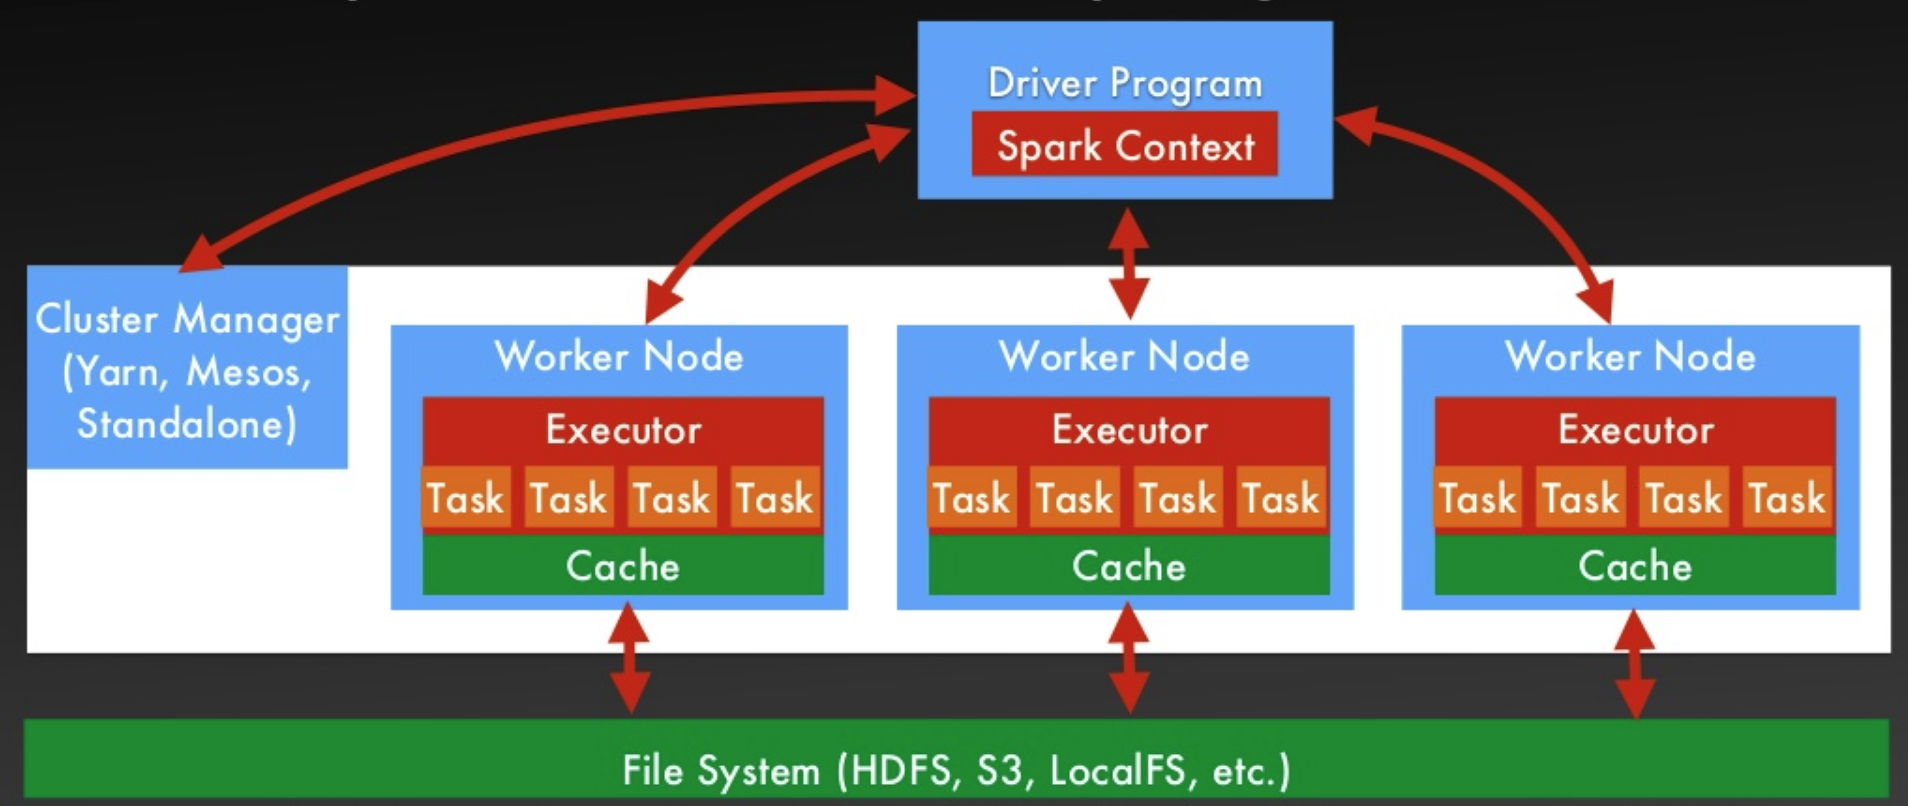
\includegraphics[scale=0.16]{figure/reduce.png}
  \end{figure}
  \begin{itemize}
    \item Spark splits the input data-set into independent chunks
    \item Chunks are processed by the workers in a completely parallel manner.
    \item This is also called MapReduce
  \end{itemize}
\end{frame}

\begin{frame}[t]{Map Reduce}
  \begin{figure}
    \centering
    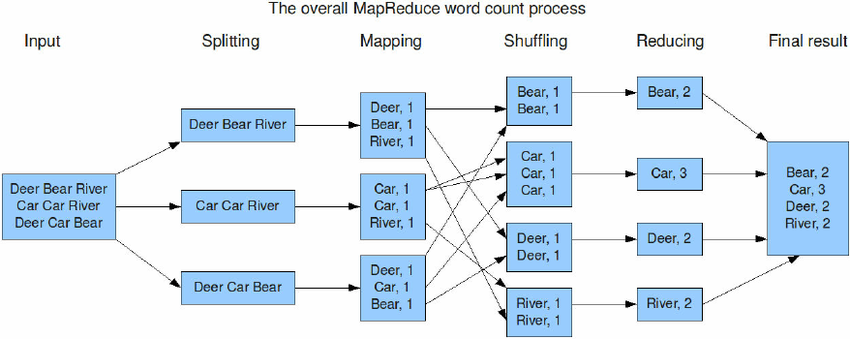
\includegraphics[scale=0.35]{figure/map_reduce.png}
  \end{figure}
 Spark retains the general idea of MapReduce from Hadoop, just not the implementation 
\end{frame}

\begin{frame}{Spark and MapReduce}
  Aim of Spark: \emph{generalize} MapReduce
  \begin{itemize}
    \item handles batch, interactive and real-time data
    \item native integration with python, Java and Scala
    \item programming at a higher level of abstraction
    \item additional constructor (next to MapReduce)
    \item more memory efficient
    \item fault tolerance
  \end{itemize}
\end{frame}

\begin{frame}[t]{General Spark Framework}
  \begin{figure}
    \centering
    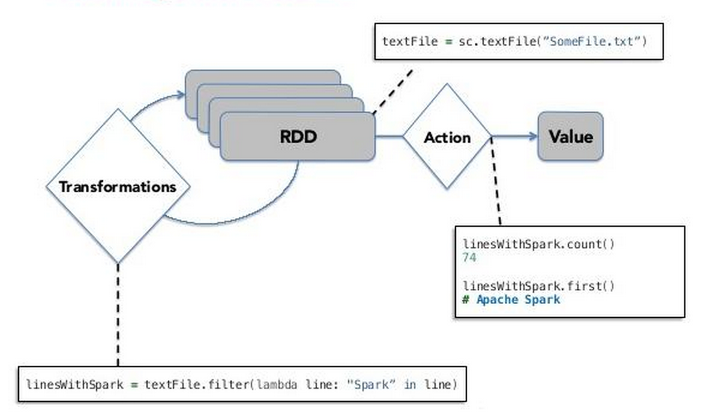
\includegraphics[scale=0.35]{figure/spark_rdd.png}
  \end{figure}
  RDD: Resilient Distributed Dataset
\end{frame}

\begin{frame}[t]{Spark Technology Stack}
  \begin{figure}
    \centering
    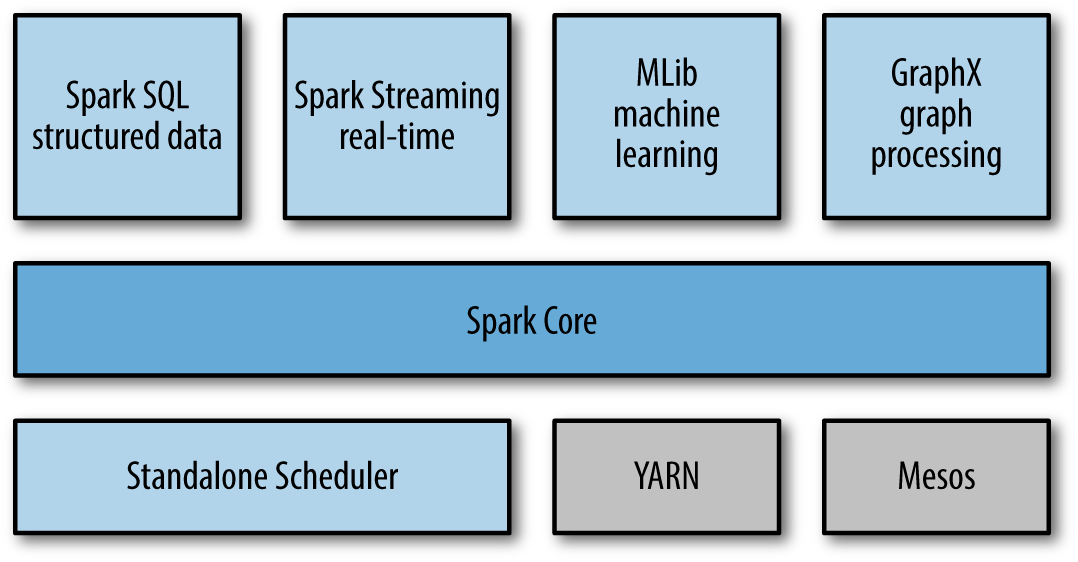
\includegraphics[scale=0.9]{figure/spark_stack.png}
  \end{figure}
\end{frame}

\begin{frame}{Application in genetics}
  Distribution of data across multiple nodes for processing by:
  \begin{itemize}
    \item Position 
    \item Sample 
  \end{itemize}
  The difference between Spark and our current approach is \textbf{scalability} and \textbf{automation}!
  \begin{itemize}
    \item Can scale to $X$ number of clusters automatically
    \item Data is dynamically chucked off and distributed
    \item Results are automatically feed back
  \end{itemize}
\end{frame}

\begin{frame}{Hail: Spark for genetic data analysis}
  Hail comes from the Neal Lab (2015) with the aim to deliver distributed algorithm to the genetic community.
  \begin{figure}
    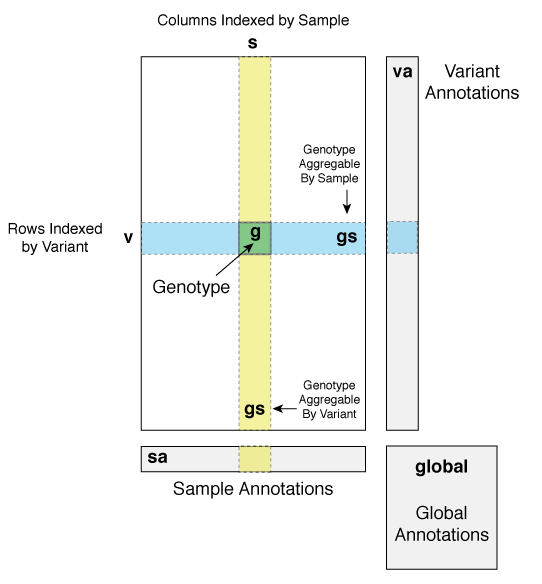
\includegraphics[scale=0.33]{figure/hail-vds-rep.png}
  \end{figure}
\end{frame}

\begin{frame}{How does it work?}
  \begin{itemize}
    \item variants are distributed in packages across spark executors \\
          E.g. Variant $rs1, \ldots, rs1000$ goes to worker $1$
    \item master organizes distribution of data packages \\
          (among current and new executors)
    \item executors perform requested computations and feed results back to master
    \item all of this is done in automation without user configuration
  \end{itemize}
\end{frame}

\begin{frame}{Using Google's Cloud}
  \textbf{Why did we use Google?}
  \begin{itemize}
    \item we got 300USD credit for free
    \item Broad pushes new versions of hail onto Google
    \item Tools are available to rapidly start a spark cluster with hail \\
          (with one simple line of code)
    \item Variant annotations are available on Google and ready to be used
  \end{itemize}
  \textbf{What are some of the cluster configurations?}
  \begin{itemize}
    \item number of workers (flexible)
    \item number or preemptive workers (flexible)
    \item number of CPU, RAM, hard disk size for each worker and master machine (fixed)
  \end{itemize}
\end{frame}

\begin{frame}[t]{Start A Hail Cluster}

  \begin{figure}
    \centering
    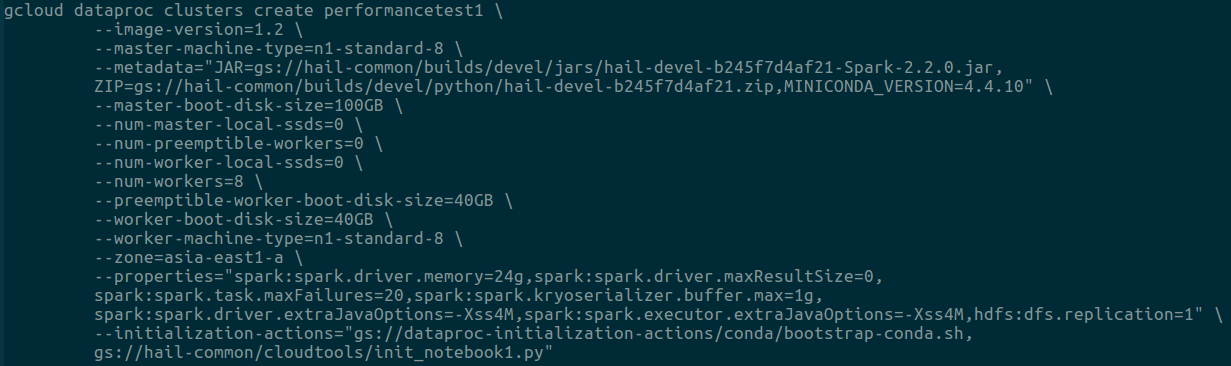
\includegraphics[scale=0.25]{figure/cluster_command.png}
  \end{figure}
  \begin{itemize}
    \item preemptive nodes: Nodes with 80\% discount
    \item MINICONDA: Python packages for scientific computing
    \item We are using a pre-build Hail version from Broad
    \item Important: Region needs to be defined
    \item Usage of standard build scripts to install Python and other tools
  \end{itemize}  
\end{frame}

\begin{frame}{Example: GWAS in Hail}
  Hail provides a high level interface to perform various tasks.
  \begin{figure}
    \centering
    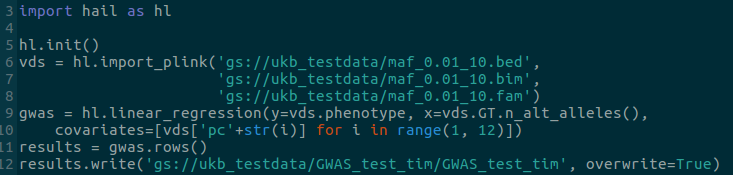
\includegraphics[scale=0.48]{figure/gwas_code.png}
  \end{figure}
  \begin{itemize}
    \item perform QC
    \item compute relationship matrix
    \item Burden tests
    \item annotations
    \item and much more
  \end{itemize}
\end{frame}


\begin{frame}{A case study}
  Lets run a simple GWAS:
  \begin{itemize}
    \item 300163 samples
    \item 369578 variant
    \item 8 workers, with each 8 CPU
  \end{itemize}
  \begin{columns}
    \begin{column}{0.5\textwidth}
      Outcome:
      \begin{itemize}
        \item CPU usage: $\sim 83\%$ \\
          Max.\ possible utilization: 87.5\%
        \item runtime: 1h 26min
        \item cost: $7.180090USD$
      \end{itemize}
    \end{column}
    \begin{column}{0.5\textwidth}
      \begin{figure}[htpb]
        \centering
        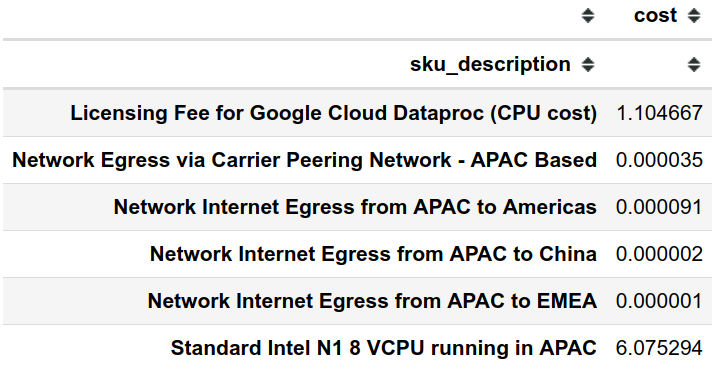
\includegraphics[width=0.99\linewidth]{figure/cost_gwas.png}
      \end{figure}
    \end{column}
  \end{columns}
  Assuming $\leq 50\%$ of workers are preemptive, a GWAS would cost not more than $83$USD (assuming 5 million SNPs)
\end{frame}

\begin{frame}{Overall cost}
  \begin{figure}[htpb]
    \centering
    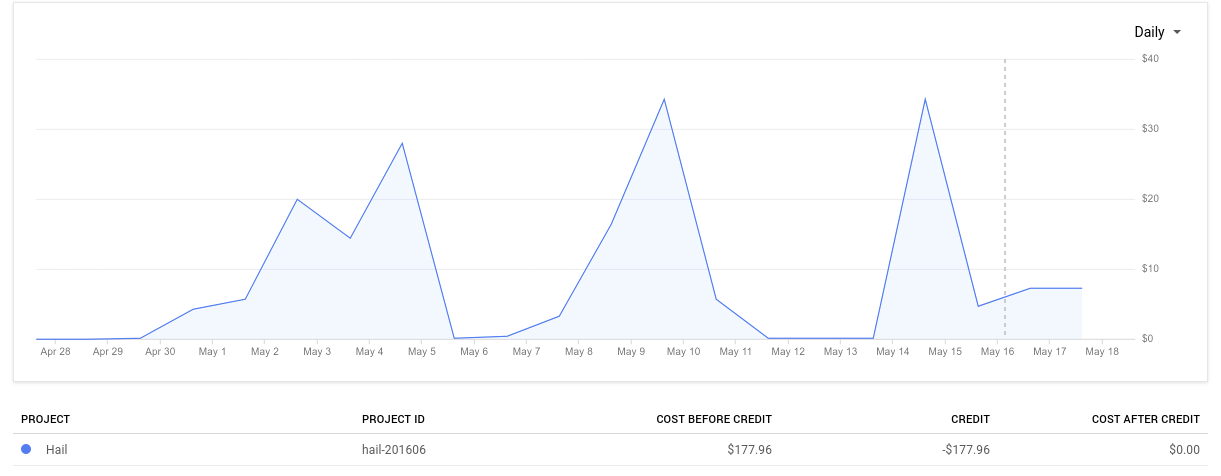
\includegraphics[width=0.9\linewidth]{figure/cash_burn.png}
  \end{figure}
  \begin{itemize}
    \item Cost control/monitoring is essential
    \item Costs are only updated every day
    \item There are a number of hidden costs (minor)
  \end{itemize}
\end{frame}

\begin{frame}[t]{Data Storage}
  \begin{itemize}
    \item We are currently paying 0.02USD per GB per Month (Buckets)
    \item Variants can also be deposited into Google's Genetic Database for much lower cost (not accessible to Spark)
    \item Data written onto the disk of master or worker nodes will be lost after cluster is shut down
  \end{itemize}
\end{frame}

\begin{frame}[t]{Overall Experience}
  \begin{itemize}
    \item More expensive than previously assumed
    \item Very, very flexible
    \item Spark allows for very fast computations
    \item Setup is less complicated than expected
    \item You get things done. Fast.
    \item Cost can be controlled by assigning fixed budgets for projects
  \end{itemize}
\end{frame}

\section{Distributed Statistical Learning}
\label{sec:distributed_statistical_learning}

\begin{frame}{Some refreshing}
  \tiny
  Lets use the simple one half mean squared error cost function: 
  \begin{equation}
    J(\theta) = \frac{1}{2m} \sum^m_{i=1} (h_{\theta}(x^{(i)}) - y^{(i)})^2
  \end{equation}
  and its partial derivative $\frac{d}{d\theta_j}J(\theta)$
  \begin{equation}
    \frac{d}{d\theta_j}J(\theta) = \frac{1}{m}\sum^{m}_{i=1}(h_{\theta}(x^{(i)})- y^{(i)})x_j^{(i)}
  \end{equation}
  which gives us the following update rule:
  \begin{equation}
    \theta_j := \theta_j - \alpha \frac{1}{400}\sum^{400}_{i=1}(h_{\theta}(x^{(i)})- y^{(i)})x_j^{(i)}
  \end{equation}

  {\large How can we parallelize this process?}

\end{frame}

\begin{frame}[t]{Parallelization}
  \small
  Let's assume we have $m=400$ samples. We could distribute these 400 across different machines

  \begin{tabular}{ll}
    Machine 1: & Use $(x^{(1)}, y^{1}),\ldots, (x^{(100)}, y^{100})$ \\
      & $temp_j^{(1)} = \sum^{100}_{i=1}(h_{\theta}(x^{(i)})- y^{(i)})x_j^{(i)}$ \\
      & \\
    Machine 2: & Use $(x^{(101)}, y^{101}),\ldots, (x^{(200)}, y^{200})$ \\
      & $temp_j^{(2)} = \sum^{100}_{i=1}(h_{\theta}(x^{(i)})- y^{(i)})x_j^{(i)}$ \\
      & \\
    Machine 3: & Use $(x^{(201)}, y^{201}),\ldots, (x^{(300)}, y^{300})$ \\
      & $temp_j^{(3)} = \sum^{100}_{i=1}(h_{\theta}(x^{(i)})- y^{(i)})x_j^{(i)}$ \\
      & \\
    Machine 4: & Use $(x^{(301)}, y^{(301)}),\ldots, (x^{(400)}, y^{400})$ \\
      & $temp_j^{(4)} = \sum^{100}_{i=1}(h_{\theta}(x^{(i)})- y^{(i)})x_j^{(i)}$
  \end{tabular}

  Then $\theta_j := \theta_j - \alpha \frac{1}{400} (temp^{(1)}_j  + temp^{(2)}_j  + temp^{(3)}_j  + temp^{(4)}_j )$
  
\end{frame}

\begin{frame}[t]{Synchronous versus asynchronous distributed training\footnote{Taken from https://www.oreilly.com/ideas/distributed-tensorflow}}
  \begin{figure}[htpb]
    \centering
    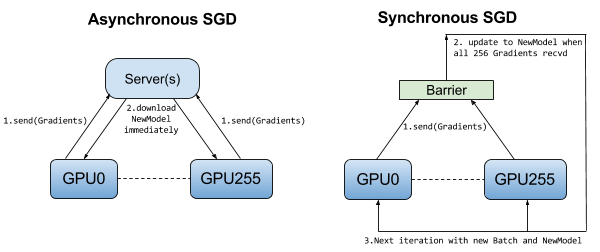
\includegraphics[width=0.8\linewidth]{figure/async_versus_synv.png}
  \end{figure}
\end{frame}

\begin{frame}[t]{Ring-allreduce}
  \begin{figure}[htpb]
    \centering
    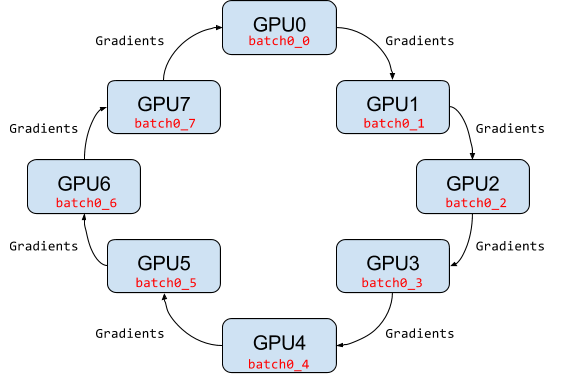
\includegraphics[width=0.8\linewidth]{figure/ring_reduce.png}
  \end{figure}
\end{frame}

\end{document}
